% Usar el tipo de documento: Artículo científico.
\documentclass[10pt,a4paper,hidelinks]{article}

% Cargar mensajes en español.
\usepackage[spanish,es-noquoting]{babel}

% Usar codificación utf-8 para acentos y otros.
\usepackage[utf8]{inputenc}
\usepackage[T1]{fontenc}
\usepackage{lmodern}

% Usar dos columnas
\usepackage{multicol}

% Separar las columnas
\setlength{\columnsep}{1cm}

% Dimensiones de los márgenes.
\usepackage[margin=1.8cm]{geometry}

% Insertar porciones de código
\usepackage{listings}

% Comenzar párrafos con separación no indentación.
\usepackage{parskip}
%enlaces
\usepackage{hyperref}
% Usar gráficos
\usepackage{graphicx}
\usepackage{caption}
\usepackage{subcaption}
%
% Usar contenedores flotantes para figuras.
\usepackage{float}

% Carpeta de las imágenes.
\graphicspath{{img/}}

% Matemáticas
\usepackage{amsmath}
\usepackage{mathtools}

% Símbolos del sistema internacional
\usepackage{siunitx}

% Dibujar circuitos electrónicos
%\usepackage[symbols]{circuitikz}
\usepackage[siunitx]{circuitikz}

% Dibujos geométricos
\usepackage{tikz}
\usetikzlibrary{through,calc,arrows,angles,babel}

\newcommand\markangle[6][red]{% [color] {X} {origin} {Y} {mark} {radius}
	% filled circle: red by default
	\begin{scope}
		\path[clip] (#2) -- (#3) -- (#4);
		\fill[color=#1,fill opacity=0.5,draw=#1,name path=circle]
		(#3) circle (#6mm);
	\end{scope}
	% middle calculation
		\path[name path=line one] (#3) -- (#2);
	\path[name path=line two] (#3) -- (#4);
	\path[%
		name intersections={of=line one and circle, by={inter one}},
		     name intersections={of=line two and circle, by={inter two}}
	] (inter one) -- (inter two) coordinate[pos=.5] (middle);
	% bissectrice definition
		\path[%
		name path=bissectrice
		] (#3) -- (barycentric cs:#3=-1,middle=1.2);
	% put mark
		\path[
		name intersections={of=bissectrice and circle, by={middleArc}}
		] (#3) -- (middleArc) node[pos=1.3] {#5};
}


\begin{document}

%\maketitle
\begin{center}
\begin{huge}
\textbf{Coco}
\end{huge}
\\[10pt]
\textbf{Rodrigo Arias Mallo}\\
rodrigo.arias@udc.es
\end{center}

\newcommand\RobotAngle{45}
\newcommand\RobotSize{2}
\newcommand\RobotRadius{4}
\newcommand\RobotThetaSonar{60.0}

\begin{multicols}{2}

\section{Descripción}
Coco es un robot diseñado para aprender los principios básicos de la robótica.
Ha sido creado con la intención de reutilizar componentes de antiguos aparatos y 
darles un nuevo uso. Así como para comprender los fundamentos teóricos
aplicados en un experimento práctico.

\subsection{Sensores}
Cuenta con varios sensores que le permiten obtener información del entorno, así
como información sobre sí mismo. Son los siguientes:

\begin{enumerate}
	% Quitar espacio entre lineas
	\setlength{\parskip}{0cm}

	\item Sensor de ultrasonidos HC-SR04
	\item Ratón de bola
	\item Sensor de luz LDR dirigido hacia delante
	\item Sensor de luz LDR ambiental
\end{enumerate}

\subsection{Motores}
Para efectuar el movimiento, dispone de dos motores Mabuchi RF-500TB-12560, colocados
a ambos lados.


\section{Calibración de sensores}
\subsection{Ultrasonidos HC-SR04}

El sensor de ultrasonidos, permite averiguar de forma estimada la posición de un obstáculo. Para ello dispone de un emisor y un receptor de ultrasonidos colocados en la misma dirección, y posicionados en la parte delantera del robot.

Para calcular la distancia del objeto, se mide el tiempo que tarda el pulso ultrasónico en viajar desde el emisor al objeto, y tras rebotar, volver al receptor.

La velocidad del sonido, depende de la temperatura del aire $\vartheta$, además
de otros
factores\footnote{\url{http://en.wikipedia.org/wiki/Speed\_of\_sound\#Practical\_formula\_for\_dry\_air}}.
Sin embargo, para una simplificación de los cálculos, se empleará la siguiente
fórmula, asumiendo que la temperatura $\vartheta$ es la misma en todas partes:
$$ v_{air} = 331.3 + 0.606\vartheta $$
Por lo tanto, si $t_e$ es el tiempo que tarda el sonido en llegar desde el emisor al obstáculo, y $t_r$ el tiempo desde el obstáculo al receptor:
$$ s_1 = v_{air} \cdot t_e $$
$$ s_2 = v_{air} \cdot t_r $$
Sin embargo, medimos $t$ que es $t_e+t_r$. Si suponemos que el robot esta parado cuando haga la medición, $s_1 = s_2$ y por tanto $t_e = t_r$. Finalmente, $s$ es la distancia del sensor al obstáculo:
\begin{equation}
	s = s_1 = s_2 = v_{air}\frac{t}{2}\label{eq:air}
\end{equation}
Es importante mencionar que $s$ no indica la posición exacta del obstáculo, si 
no la distancia del mismo al sensor.

\subsubsection{Ángulo de apertura $\theta_{sonar}$}
Para calibrar el sensor, es necesario determinar el ángulo de apertura 
$\theta_{sonar}$, que indica hasta que punto el sensor puede recibir el eco del 
sonido. De modo que se realizarán una serie de experimentos, que indicarán de 
forma experimental dicho ángulo. En la figura~\ref{fig:sonar} se observa un
esquema del experimento.

Primero un objeto se coloca en el campo de visión del sensor, en $C_1$. Luego se 
desplaza hacia $A_2$, siguiendo una trayectoria circular centrada en $O$, y se 
observa el ángulo $\theta_1$ en el que deja de observarse dicho objeto. De igual 
modo se repite en el otro sentido, y se calcula el ángulo $\theta_{2}$.

Dado que el sonar puede no estar centrado, se anotarán las medidas de $\theta_1$
y $\theta_2$, para luego estimar $\theta_{sonar}$.

\begin{center}
\begin{tikzpicture}[>=latex]

	\pgfmathsetmacro{\SonarS}{6}
	\pgfmathsetmacro{\Obstacle}{1}
	\pgfmathsetmacro{\RobotSemiTheta}{\RobotThetaSonar/2.0}
    \pgfmathsetmacro{\RobotBall}{0.15}%
    \pgfmathsetmacro{\RobotOC}{sqrt(\RobotSize*\RobotSize + \RobotRadius*\RobotRadius)}%
    \pgfmathsetmacro{\RobotAngleAOC}{atan(\RobotSize/\RobotRadius)}%
    \def\BallBeta{\RobotAngleAOC}
        
    
    \fill [black] (0,0) coordinate [label=left:$O$] (O) circle (1pt);
    \coordinate (X) at (\SonarS/4,0);
    \fill [black] (-\RobotThetaSonar/2:\SonarS) coordinate [label=right:$A_1$] (A1) circle (1pt);
    \fill [black] (\RobotThetaSonar/2:\SonarS) coordinate [label=right:$A_2$] (A2) circle (1pt);
        \fill [black] (\RobotThetaSonar/4:\SonarS) coordinate [label=right:$C_1$] (C1) circle (1pt);
        \fill [black] (\RobotThetaSonar*3/4:\SonarS) coordinate [label=right:$C_2$] (C2) circle (1pt);
%    \fill (A1) +(0,-\RobotSize) coordinate [label=below:$C_1$] (C1) circle (1pt);
%    \fill[rotate=\RobotAngle] (A2) +(0,-\RobotSize) coordinate [label=above:$C_2$] (C2) circle (1pt);

	%(-\RobotThetaSonar/2:30:\SonarS) node[pos=0.5,auto=right]{$a$};

	% Pintar objeto 1
	\draw[dotted,rotate=\RobotThetaSonar/4] (C1) +(0,\Obstacle/2) rectangle +(\Obstacle,-\Obstacle/2);

	% Pintar objeto 2
	\draw[dotted,rotate=\RobotThetaSonar*3/4] (C2) +(0,\Obstacle/2) rectangle +(\Obstacle,-\Obstacle/2);
    
    \draw (O) -- (A1);
    \draw (O) -- (A2);
    \draw[dotted] (O) -- (X);
    %\draw[dotted] (O) -- (C1);

	%Dibujar arco del campo de visión
	\draw[dotted] (A2) arc[
		start angle=\RobotThetaSonar/2,
		delta angle=-\RobotThetaSonar,
		radius=\SonarS];
	
	% Pintar el vector s
	%\draw[red,-latex,shorten >=1pt] (O) -- (C1)
	%	node[pos=0.5,auto=left]{$\vec{s}$};
	\draw[red] (O) -- (C1)
		node[pos=0.5,auto=left]{$s$};
    
	% Ángulos
	\begin{scope}
		\path[clip] (A1) -- (O) -- (A2) -- cycle;
		%\draw [red, fill=red!20] (O) circle (1.5);
		\draw [dotted] (O) circle (\SonarS/3);
		\node[right] at ($(O) +(\SonarS/3, 0)$) {$\theta_{sonar}$};

		\draw [dotted] (O) circle (\SonarS/5);
		\node[right] at ($(O) +(\RobotThetaSonar/4:\SonarS/5)$) {$\theta_1$};
		\node[right] at ($(O) +(-\RobotThetaSonar/4:\SonarS/5)$) {$\theta_2$};
	\end{scope}


		
    
    % Ángulos
    %\draw[red] (\RobotRadius/5,0) arc (0:\RobotAngle:\RobotRadius/5.0) node[pos=0.5,auto=right]{$\theta_{sonar}$};
    %\draw[dotted] (\RobotRadius/5,0) arc (0:-\RobotAngleAOC:\RobotRadius/5.0) node[pos=0.5,auto=left]{$\beta$};
    %\draw[dotted] (A1) +(-\RobotRadius/5,0) arc (180:90+\RobotAngle/2:\RobotRadius/5.0) node[pos=0.5,auto=left]{$\gamma$};
    
    % Dibujar el robot en A1
    %\draw[dotted] (A1) +(-\RobotSize/2,0) rectangle +(\RobotSize/2,-\RobotSize);
    %\draw[dotted] (C1) circle(\RobotBall);
    
    %Dibujar el robot en A2
    %\draw[dotted,rotate=\RobotAngle] (A2) +(-\RobotSize/2,0) rectangle +(\RobotSize/2,-\RobotSize);
    %\draw[dotted] (C2) circle(\RobotBall);
    
   	%Trayectoria raton
   	%\pgfmathsetmacro{\XValueArc}{\ArcRadius*cos(\ArcAngle)}%
   	%\draw[blue] (C1) arc (-\RobotAngleAOC:\RobotAngle-\RobotAngleAOC:\RobotOC) node[pos=0.5,auto=right]{$a$};
    
    %\draw (0,0) coordinate [label=right:$O$] (O) circle(4);
    %\draw[dotted] (A1) arc (0:\RobotAngle:\RobotRadius);
    %\draw[-latex,shorten >=1pt] (A1) -- (A2) node[pos=0.5,auto=right]{$\vec{r}$};
    
    %Dibujar el vector del raton
    %\draw[red,-latex,shorten >=1pt] (C1) -- +(90-\RobotAngleAOC:\RobotRadius/3) node[pos=0.5,auto=right]{$\vec{m}$};
    
    
\end{tikzpicture}
\captionof{figure}{Sensor de ultrasonido.\label{fig:sonar}}
\end{center}


Tras realizar las mediciones, se obtienen los siguientes resultados.
\begin{center}
\begin{tabular}{ | c | c | c | }
\hline
$s$ & $\theta_1$ & $\theta_2$ \\ \hline
m    &  º &  º \\ \hline \hline
0.20 & 30 & 27 \\ \hline
0.30 & 30 & 27 \\ \hline
0.40 & 31 & 28 \\ \hline
0.50 & 28 & 26 \\ \hline
0.60 & 30 & 28 \\ \hline
0.80 & 31 & 29 \\ \hline
1.00 & 29 & 29 \\ \hline
1.20 & 30 & 28 \\ \hline \hline
media& 29.875 & 27.75 \\ \hline
\end{tabular}
\end{center}

Se empleará la media de los valores de los ángulos, para reducir los errores que
se pudieran producir en las medidas de los mismos, quedando $\theta_1 = 29.875
º$ y $\theta_2 = 27.75 º$.

Por lo tanto ya se puede obtener el ángulo de apertura:
$$\theta_{sonar} = \theta_1 + \theta_2 = 57.625 º $$

\subsubsection{Distancia medida}

Para completar la calibración, es necesario poder calcular la distancia $s$,
sabiendo el tiempo $t$. Para ello, se realizará otro experimento, midiendo las
distancias de forma manual $s_r$ con una regla, y comparándolas con el valor
teórico $s_t$, calculado con la ecuación~\ref{eq:air}.

\begin{center}
\begin{tabular}{ | c | c | c | }
\hline
$s_{r}$ & $s_{t}$ & $t$ \\ \hline
m & m & \si{\micro\second} \\ \hline \hline
0.20 & 0.138 &  805 \\ \hline
0.30 & 0.210 & 1225 \\ \hline
0.40 & 0.281 & 1638 \\ \hline
0.50 & 0.353 & 2060 \\ \hline
0.60 & 0.429 & 2500 \\ \hline
0.80 & 0.568 & 3305 \\ \hline
1.00 & 0.713 & 4155 \\ \hline
1.20 & 0.859 & 5000 \\ \hline
\end{tabular}
\end{center}

Se observa que el valor teórico $s_t$, no coincide con el valor real medido 
$s_r$.

Sería posible solucionar el problema empleando una corrección del error. Para 
ello se emplea una regresión lineal. Con Octave, \texttt{polyfit} muestra los 
coeficientes de la recta:
\begin{center}
\texttt{2.3864e+02   7.8846e-03}
\end{center}
Cuya recta (rojo) se puede observar en la figura~\ref{fig:sonar_plot}. Su 
ecuación es:
$$s = 238.64t + 7.8846\cdot10^{-3}$$
\begin{center}
%	\includegraphics[width=0.8\textwidth]{image.png}
	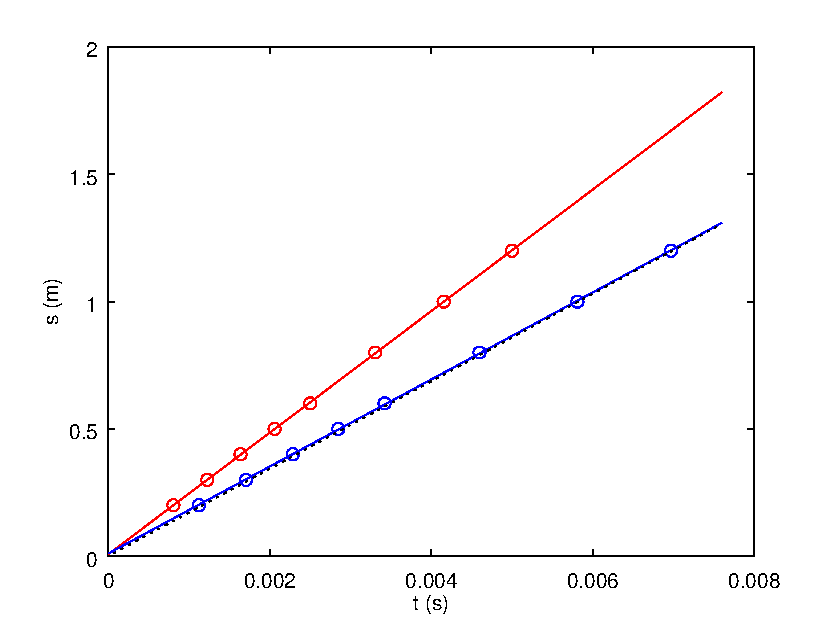
\includegraphics[scale=0.58]{sonar.pdf}
	\captionof{figure}{Valores experimentales erróneos (rojo) y correctos 
(azul). La recta punteada es el valor teórico.\label{fig:sonar_plot}}
\end{center}

Después de repasar el programa que muestra el tiempo en Arduino, resulta que la 
función \texttt{pulseIn} calcula el tiempo que ha pasado, empleando un bucle, y 
luego multiplica las vueltas del bucle por el número de instrucciones. Sin 
embargo, el compilador \texttt{avr-gcc} puede alterar este número cuando se 
aplican optimizaciones. Este problema, provoca que el tiempo se vea alterado de 
la forma $ t_{real} = t * K $. Siendo $ K = 1.3898 $, hallado de forma 
experimental.

Tras programar una nueva biblioteca para emplear el sensor de ultrasonidos, de 
forma independiente a las optimizaciones del código, y empleando las 
interrupciones, se vuelven a realizar las medidas.

%Para calcular el tiempo se realizan 100000 mediciones y se halla la media.

\begin{center}
\begin{tabular}{ | c | c | c | }
\hline
$s_{r}$ & $s_{t}$ & $t$\\ \hline
m & m & \si{\micro\second} \\ \hline \hline
0.20 & 0.193 & 1122 \\ \hline
0.30 & 0.293 & 1705 \\ \hline
0.40 & 0.392 & 2285 \\ \hline
0.50 & 0.489 & 2848 \\ \hline
0.60 & 0.588 & 3422 \\ \hline
0.80 & 0.789 & 4597 \\ \hline
1.00 & 0.998 & 5810 \\ \hline
1.20 & 1.197 & 6970 \\ \hline
\end{tabular}
\end{center}

Obteniendo por regresión lineal, de la misma forma, los coeficientes:
\begin{center}
\texttt{1.7084e+02   1.0857e-02}
\end{center}
Y por tanto, la recta característica es:
$$ s = 170.84 t + 1.0857\cdot 10^{-2} = 341.68\frac{t}{2} + 1.0857\cdot 10^{-2}
$$

Si la comparamos con la ecuación~\ref{eq:air}, se puede observar que es muy 
similar a lo esperado.

La velocidad del sonido calculada de forma experimental, resulta ser 341.68 m/s.  
Este valor puede oscilar, ya que depende de la temperatura. Para calcular la 
temperatura:
$$ \vartheta = \frac{v_{air}-331.3}{0.606} = 17.129 \si{\celsius} $$
Dado que el experimento se ha realizado por la noche, esa temperatura se 
encuentra dentro de un margen adecuado. La temperatura medida por un termómetro 
en la habitación es de 18 ºC. Por lo que se puede afirmar que el experimento 
muestra unos resultados esperados.

Existe un error fijo de aproximadamente un centímetro, que se debe a la 
dificultad de centrar la regla en el centro del sensor de ultrasonidos. Sin 
embargo, para determinar la distancia de un objeto al robot, esta distancia es 
despreciable.

Es importante mencionar, que un ajuste del error, empleando un método de 
regresión, permite esconder errores como el que ha sido detectado y corregido.  
Por ello, se ha decidido emplear los cálculos teóricos, y si no concuerdan con 
los esperados, averiguar que ha causado el error.

\subsection{LDR}

El sensor LDR permite obtener una medida de la cantidad de luz que incide sobre
el mismo. El robot dispone de dos sensores LDR. Uno ambiental, está colocado en
la parte superior, orientado hacia arriba. Además está cubierto por un cilindro
cerrado de 4cm de plástico blanco. Esto le permite obtener una medida de la luz
ambiente sin importar la dirección de donde proviene.

El sensor LDR direccional, se encuentra en la parte delantera orientado al 
frente. Este sin embargo, está encapsulado en un cilindro abierto, de caucho 
negro mate. Lo cual le permite observar de forma direccional la luz que recibe 
por el frente, con el objetivo de encontrar una luz.

\subsubsection{LDR ambiental}

Para calibrar el sensor ambiental, se realizarán algunas medidas comparando la 
distancia a un foco de luz, y la invarianza de la orientación.

964

El valor medido por el sensor, está representado en un intervalo $[0, 1024)$ de 
valores discretos. El valor 0, corresponde con un voltaje de 0V en la entrada de 
Arduino, y 1023 con +5V.
$$ V_0 = 5 \cdot \frac{l_0}{1023} $$
En la figura~\ref{fig:ldr_circuito} se observa el montaje del LDR $R_2$, junto 
con otra resistencia $R_1$ de un valor fijo de $10\si{\kohm}$.

\begin{center}
\begin{tikzpicture}
	\draw
		(0,0) to ++(0,-1) node[ground] {}
		(0,0) to[R, l_=$R_1$, -*] ++(2,0)
		to[short, -o] ++(0,-1) node[below] {$V_0$}
		
		(2,0) to[phR, l_=$R_2$] ++(2,0)
		to[short, -o] ++(0, -1) node[below] {V}
	;
\end{tikzpicture}
\captionof{figure}{Circuito del sensor LDR.\label{fig:ldr_circuito}}
\end{center}

Para calcular el voltaje en $V_0$:
$$ I = \frac{V}{R_T} = \frac{V}{R_1 + R_2} $$
$$ V_{0} = I \cdot R_1 = V \frac{R_1}{R_1+R_2} = \frac{V}{1+\frac{R_2}{R_1}}$$
Y posteriormente el valor de $R_2$:
$$ R_{2} = R_1 \frac{V-V_0}{V_0}$$
La relación entre la iluminación $E$ y la resistencia $R$ viene dada 
por\footnote{\url{http://www.brighton-webs.co.uk/electronics/light\_dependent\_resistor.aspx}}:
$$ \frac{E_2}{E_1} = \left(\frac{R_2}{R_1}\right)^\gamma$$
Y entre la distancia $D$ y la iluminación:
$$ \frac{E_1}{E_2} = \left(\frac{D_2}{D_1}\right)^2$$
De forma que, para calcular el parámetro $\gamma$:
$$ E_2 = E_1 \cdot \left( \frac{R_2}{R_1} \right) ^\gamma \Rightarrow 
\left(\frac{R_2}{R_1} \right)^{-\gamma} = \left(\frac{D_2}{D_1}\right)^2$$
$$ \gamma = \frac{2 \ln \frac{D_2}{D_1} }{-\ln\frac{R_2}{R_1}} $$

% TODO: Comprobar estas ecuaciones por algún libro.
\begin{center}
\begin{tabular}{ *{8}{|c} | }
\hline
$s_{r}$ & 0.20 & 0.30 & 0.40 & 0.60 & 0.80 & 1.00 & 1.20 \\ \hline
ldr & 500 & 394 & 330 & 255 & 202 & 160 & 140 \\ \hline
\end{tabular}
\end{center}

\subsection{Ratón}

En la parte posterior, un ratón de bola permite obtener mediciones del movimiento del
robot. Tiene un controlador EM83702BP, que dispone con dos contadores digitales que
realizan la medición del desplazamiento en el eje $x$ e $y$.

Una bola de goma se encuentra en contacto con el suelo. Al desplazar el ratón, 
la bola gira alrededor de un eje imaginario, que es perpendicular al sentido del
desplazamiento y paralelo al suelo.

Ya que los movimientos efectuados por el robot serán los que provoquen sus dos ruedas,
se puede determinar la posición, midiendo sólo el desplazamiento del ratón. Para ello,
se observa en la figura~\ref{fig:giro} un ejemplo de un giro de $\alpha = \RobotAngleº$.

\begin{center}
\begin{tikzpicture}[>=latex]
    %\path[draw] (-4,0)  coordinate [label= left:$A$] (A)
    %        -- ( 0,4)  coordinate [label=above:$C$] (C)
    %        -- ( 4,0)  coordinate [label=right:$B$] (B)
    %        -- cycle;
    %\foreach \point in {A,B,C}
    %       \fill [black] (\point) circle (2pt);
    %\draw [color=red] circle(4cm);
    
    
    %\draw (A) rectangle (1,1);
    
    %\def\robotsize{(1,1)}
    %\pgfmathsetmacro{\RobotSize}{2.0}%
    %\pgfmathsetmacro{\RobotAngle}{-45.0}%
    %\pgfmathsetmacro{\RobotRadius}{6.0}%
    \pgfmathsetmacro{\RobotBall}{0.15}%
    \pgfmathsetmacro{\RobotOC}{sqrt(\RobotSize*\RobotSize + \RobotRadius*\RobotRadius)}%
    \pgfmathsetmacro{\RobotAngleAOC}{atan(\RobotSize/\RobotRadius)}%
    \def\BallBeta{\RobotAngleAOC}
        
    
    \fill [black] (0,0) coordinate [label=left:$O$] (O) circle (1pt);
    \fill [black] (0:\RobotRadius) coordinate [label=below:$A_1$] (A1) circle (1pt);
    \fill [black] (\RobotAngle:\RobotRadius) coordinate [label=above:$A_2$] (A2) circle (1pt);
    \fill (A1) +(0,-\RobotSize) coordinate [label=below:$C_1$] (C1) circle (1pt);
    \fill[rotate=\RobotAngle] (A2) +(0,-\RobotSize) coordinate [label=above:$C_2$] (C2) circle (1pt);
    
    
    \draw[dotted] (O) -- (A1);
    \draw[dotted] (O) -- (A2);
    \draw[dotted] (O) -- (C1);
    
    % Ángulos
    \draw[dotted] (\RobotRadius/5,0) arc (0:\RobotAngle:\RobotRadius/5.0) node[pos=0.5,auto=right]{$\alpha$};
    \draw[dotted] (\RobotRadius/5,0) arc (0:-\RobotAngleAOC:\RobotRadius/5.0) node[pos=0.5,auto=left]{$\beta$};
    \draw[dotted] (A1) +(-\RobotRadius/5,0) arc (180:90+\RobotAngle/2:\RobotRadius/5.0) node[pos=0.5,auto=left]{$\gamma$};
    
    % Dibujar el robot en A1
    \draw[dotted] (A1) +(-\RobotSize/2,0) rectangle +(\RobotSize/2,-\RobotSize);
    \draw[dotted] (C1) circle(\RobotBall);
    
    %Dibujar el robot en A2
    \draw[dotted,rotate=\RobotAngle] (A2) +(-\RobotSize/2,0) rectangle +(\RobotSize/2,-\RobotSize);
    \draw[dotted] (C2) circle(\RobotBall);
    
   	%Trayectoria raton
   	%\pgfmathsetmacro{\XValueArc}{\ArcRadius*cos(\ArcAngle)}%
   	\draw[blue] (C1) arc (-\RobotAngleAOC:\RobotAngle-\RobotAngleAOC:\RobotOC) node[pos=0.5,auto=right]{$a$};
    
    %\draw (0,0) coordinate [label=right:$O$] (O) circle(4);
    \draw[dotted] (A1) arc (0:\RobotAngle:\RobotRadius);
    \draw[-latex,shorten >=1pt] (A1) -- (A2) node[pos=0.5,auto=right]{$\vec{r}$};
    
    %Dibujar el vector del raton
    \draw[red,-latex,shorten >=1pt] (C1) -- +(90-\RobotAngleAOC:\RobotRadius/3) node[pos=0.5,auto=right]{$\vec{m}$};
    
    
\end{tikzpicture}
\captionof{figure}{Diagrama de un giro del robot.\label{fig:giro}}
\end{center}

El vector $ \vec{r} $ indica el movimiento que realizó el robot en línea recta.
Conociendo el ángulo $\gamma$:
$$ R' = \overline{OA_1} \quad R = \overline{OC_1} $$
$$
r_x = \begin{cases}
		R'(1-\cos \gamma) & \text{si } \gamma < 0\\
		-R'(1-\cos \gamma) & \text{si } \gamma > 0\\
		0 & \text{si } \gamma = 0\\
	\end{cases}
$$
$$
r_y = \begin{cases}
		-R'(\sin \gamma) & \text{si } \gamma < 0\\
		R'(\sin \gamma) & \text{si } \gamma > 0\\
		m_x & \text{si } \gamma = 0\\
	\end{cases}
$$
\subsubsection{Movimiento de la bola}
Para poder analizar el movimiento que realizará el robot, mediante la 
información que este proporciona, es necesario conocer como varía el vector 
$\vec{m}$ con respecto a la información proporcionada por los optocodificadores.

De modo que se analiza a continuación, como el movimiento de la bola, roza en 
los puntos $Bx$ y $By$ con los rodillos del ratón. En la figura~\ref{fig:bola} 
se observa con detalle el mismo giro que en la figura~\ref{fig:giro}.
\\
\\
\\
\\
\\
\\
\\
\\
\\
\\

% TODO: Poner los ejes en la figura y R

\begin{center}
\begin{tikzpicture}[>=latex]
	\pgfmathsetmacro{\BallRadius}{3.0}%
	\pgfmathsetmacro{\BallOptoL}{2}%
	\pgfmathsetmacro{\BallOptoD}{0.5}%
	\pgfmathsetmacro{\BallBeta}{atan(\RobotSize/\RobotRadius)}%
	\pgfmathsetmacro{\BallBetaDouble}{90.0-\BallBeta*2.0}%

	\draw circle(\BallRadius);
	\fill [black] (0,0) coordinate [label=below:$O$] (O) circle (1pt);
	%Puntos de choque
	\fill [black] (0,-\BallRadius) coordinate [label=below:$B_x$] (Bx) circle (1pt);
	\fill [black] (-\BallRadius,0) coordinate [label=left:$B_y$] (By) circle (1pt);
	%Ejes
	\draw[dotted] (-\BallRadius,0) -- (\BallRadius,0);
	\draw[dotted] (0,\BallRadius) -- (0,-\BallRadius);
	%Cilindros de los ejes
	\draw[dotted] (By) +(-\BallOptoD,-\BallOptoL) rectangle +(0,\BallOptoL);
	\draw[dotted] (Bx) +(-\BallOptoL,-\BallOptoD) rectangle +(\BallOptoL,0);
	%Puntos
	\fill[black] (180-\BallBeta*2:\BallRadius) coordinate [label=above:$C_y$] (Cy) circle (1pt);
	\draw[blue] (By) -- (Cy) node[pos=0.5,auto=right]{$d_y$};
	\fill[black] (90-\BallBeta*2:\BallRadius) coordinate [label=right:$C_x$] (Cx) circle (1pt);
	\draw[blue] (Bx) -- (Cx) node[pos=0.5,auto=right]{$d_x$};
	%Ángulos
	%\draw[dotted] (Bx) +(-90:\BallRadius/5) arc
	%(-90:-90-\BallBeta:\BallRadius/5.0) node[pos=0,auto=left]{$\beta$};

	%\draw[dotted,rotate=90-\BallBeta]
	%	($0.5*(By)+0.5*(Cy)$) ellipse (1.35 and 0.15)
	%	($0.5*(Bx)+0.5*(Cx)$) ellipse (2 and 0.15);
	%\coordinate (C3) at ($0.5*(C1)+0.5*(C2)$)


	% Angulos del eje x
	\begin{scope}
		\path[clip] (Bx) -- (O) -- (Cx) -- cycle;
		\draw (Bx) circle (\BallRadius/3);
		\node[above] at ($(Bx) +(+90-\BallBeta/2:\BallRadius/3)$) {$\beta$};
		\draw (O) circle (\BallRadius/5);
		\node[right] at ($(O) +(-\BallBeta:\BallRadius/5)$) {$\gamma$};
	\end{scope}

	%Ángulos del eje y
	\begin{scope}
		\path[clip] (By) -- (O) -- (Cy) -- cycle;
		\draw (By) circle (\BallRadius/5);
		\node[right] at ($(By) +(+45-\BallBeta/2:\BallRadius/5)$) {$\delta$};
		\draw (O) circle (\BallRadius/5);
		\node[left] at ($(O) +(+180-\BallBeta:\BallRadius/5)$) {$\theta$};
	\end{scope}

	%Dibujar el vector del raton
	\draw[red,-latex,shorten >=1pt] (O) -- +(90-\BallBeta:\BallRadius/2)
		node[pos=0.5,auto=left]{$\vec{m}$};

	\draw[dotted] (O) -- (Cx);
	%\draw[dotted] (Cx) +(270.0-\BallBeta:\BallRadius/5) arc (90.0-\BallBeta:\BallBetaDouble:\BallRadius/5.0) node[auto=right]{$\beta$};

	%\draw[dotted] (O) +(\BallBetaDouble:\BallRadius/4.0) arc (\BallBetaDouble:-90.0:\BallRadius/4.0) node[auto=right,pos=0.5]{$\delta$};

	\draw[dotted] (O) -- (Cy);
	%\draw[dotted] (O) +(90.0+\BallBetaDouble:\BallRadius/6.0) arc (90.0+\BallBetaDouble:180.0:\BallRadius/6.0) node[auto=above]{$\theta$};
	%node[auto=left,pos=0.5]{$\theta$}



\end{tikzpicture}
\captionof{figure}{Diagrama de la bola del ratón. Los ejes están 
invertidos.\label{fig:bola}}
\end{center}

\subsubsection{El tamaño de la bola}

A continuación, trataré de averiguar cómo se mueven los rodillos del ratón, 
cuando la bola gira. Para ello moveré el ratón un desplazamiento $\vec{m}$ a una 
velocidad uniforme y en línea recta.

Los ejes están intercambiados con respecto al orden habitual de un plano. Esto 
es debido a que el ratón está colocado en el robot como en la figura. Sin 
embargo mantienen el sentido. Hacia arriba y derecha son positivos.

El rodillo inferior, girará rozando continuamente por el punto $B_x$ a medida 
que la bola gire. Dado que la dirección $\vec{m}$ permanece constante durante 
este movimiento, el punto $B_x$ describirá una trayectoria circular en la 
superficie de la bola. La bola tiene un radio $R_b$.

Llamo $p_x$ al perímetro de esta circunferencia, que es tangente a $B_x$ y $C_x$ 
y que tiene por diámetro $d_x$. De modo que cuando la bola dé una vuelta 
completa, el rodillo habrá avanzado exactamente $p_x$.

La distancia $d_x$ es la cuerda de ángulo $\gamma$, cuya longitud es, por su 
propia definición:
$$ d_x = R_b \, \text{crd} \, \gamma = 2R_b \sin \frac{\gamma}{2}$$
Además, el ángulo $\gamma = 180º - 2\beta$, pues forma un triángulo isósceles:
$$ d_x = 2R_b \sin(90-\beta) = 2R_b\cos \beta$$
De igual modo para $d_y$:
$$ d_y = R_b \, \text{crd} \, \theta = 2R_b \sin \frac{\theta}{2} $$
Sabiendo que $\theta = 180º - 2\delta$ y que $\beta = 90 - \delta$, puesto que 
$d_x \parallel d_y$:
$$ d_y = 2R_b \sin (90 - \delta) = 2R_b \sin \beta $$
Finalmente, para los perímetros:
$$ p_x = \frac{2\pi d_x}{2} = 2 \pi R_b\cos \beta \quad  p_y = \frac{2\pi 
d_y}{2} = 2 \pi R_b\sin \beta $$

Si suponemos que no hay ningún deslizamiento entre la bola y el rodillo, cuando 
la bola avance $\vec{m}$, girará un ángulo $\theta_b$:
$$ \theta_b = \frac{m}{R_b} $$

Si $R_r$ es el radio de los rodillos, estos girarán un ángulo:
$$ \theta_x = \frac{\theta_b d_x}{2R_r} \quad
	\theta_y = \frac{\theta_b d_y}{2R_r}$$
Sustituyendo $d_x$ y $d_y$:
$$ \theta_x = \frac{\theta_b 2R_b\cos \beta}{2R_r} =
	\frac{R_b}{R_r}\theta_b\cos \beta$$
$$ \theta_y = \frac{\theta_b 2R_b\sin \beta}{2R_r} =
	\frac{R_b}{R_r}\theta_b\sin \beta$$
Recuperando el valor de $\theta_b$, el radio $R_b$ dasaparece:
$$ \theta_x = \frac{m \cos \beta}{R_r} \quad
\theta_y = \frac{m \sin \beta}{R_r} $$
Es decir, que el tamaño no importa, de la bola.

\subsubsection{Los optoreceptores}

Los rodillos que rozan con la bola, tienen en los extremos unos discos con
ranuras equiespaciadas, de modo que cortan un haz de luz infrarrojo al girar.  
Este efecto, provoca que un sensor registre el número de veces que se ha cortado 
el haz, y por lo tanto mide, de forma discreta, cuánto ha girado el rodillo, es 
decir $\theta_x$ y $\theta_y$.

Cada disco tiene 27 dientes y $R_r$ mide 1.35$\pm$0.1 mm.

$o_x$ y $o_y$ son los valores medidos por los contadores que acumulan el número 
de veces que se ha cortado el haz, y por lo tanto el número de dientes que se ha 
desplazado el rodillo.

$$o_x = \frac{27 \theta_x}{2\pi} \quad o_y = \frac{27 \theta_y}{2\pi}$$

Sustituyendo el valor del ángulo $\theta_x$ y $\theta_y$:
$$ o_x = \frac{27}{2 \pi R_r} m \cos \beta \quad
	o_y = \frac{27}{2 \pi R_r} m \sin \beta $$


\section{Posibles errores}

La función \texttt{attachInterrupt} no borra las banderas (flags) \texttt{INTF0} 
y \texttt{INTF1} del registro \texttt{EIFR}, de forma que al colocar una 
interrupción por primera vez, es posible que se ejecute al comienzo sin haber 
recibido tal interrupción. Una posible solución es añadir esta línea al comienzo 
de la función:

\texttt{EIFR |= \_BV(INTF0) || \_BV(INTF1);}

La función \texttt{pulseIn} calcula el tiempo dependiendo de las optimizaciones
que se produzcan. Es necesario que sea independiente. Además es conveniente
sustituirla por alguna función no bloqueante que emplee interrupciones.

%\vfill


\end{multicols}
\end{document}
